\documentclass[aspectratio=43]{beamer}

\usepackage[utf8]{inputenc}

\usepackage{amsfonts}
\usepackage{amsmath}
\usepackage{color}
\usepackage{listings}
\usepackage{tikz}
\usepackage{hyperref}

\usetheme{Rochester}
\usecolortheme{beaver}

\addtobeamertemplate{navigation symbols}{}{%
    \usebeamerfont{footline}%
    \usebeamercolor[fg]{footline}%
    \hspace{1em}%
    \insertframenumber/\inserttotalframenumber
}

\lstloadlanguages{C++}
    \lstset{%
        language={C++},
        basicstyle=\ttfamily,
        keywordstyle=\color{blue},
        showstringspaces=false,
        escapechar={§},
        escapeinside=||
    }

\newif\iftransitions
 \transitionstrue


\newif\iffast
% \fasttrue

\title{The deal with \texttt{-ffast-math}}
%\subtitle{No subtitle}
\author{Andreas Weis}
\institute{BMW AG}
\date{MUC++, June 26, 2018}


\begin{document}

\frame{\titlepage}


\begin{frame}[fragile]
  \frametitle{Previously on this channel...}
    \begin{lstlisting}
double calc(std::vector<double> const& vd)
{
  double acc = 0.0;
  for(auto const& d : vd) {
    acc += d * d;
  }
  return acc;
}
    \end{lstlisting}
\end{frame}

\begin{frame}[fragile]
  \frametitle{Previously on this channel...}
    \begin{lstlisting}
double calc(std::vector<double> const& vd)
{
  return std::inner_product(begin(vd), end(vd),
                            begin(vd), 0.0);
}
    \end{lstlisting}
\end{frame}

\begin{frame}[fragile]
  \frametitle{Previously on this channel...}
    \begin{lstlisting}
double calc(std::vector<double> const& vd)
{
  double acc = 0.0;
  for(size_t i = 0; i < vd.size(); i += 2) {
    acc += vd[i]     * vd[i];
    acc += vd[i + 1] * vd[i + 1];
  }
  return acc;
}
    \end{lstlisting}
\end{frame}

\begin{frame}[fragile]
  \frametitle{Previously on this channel...}
    \begin{lstlisting}
double calc(std::vector<double> const& vd)
{
  double acc1 = 0.0, acc2 = 0.0;
  for(size_t i = 0; i < vd.size(); i += 2) {
    acc1 += vd[i]     * vd[i];
    acc2 += vd[i + 1] * vd[i + 1];
  }
  return acc1 + acc2;
}
    \end{lstlisting}
\end{frame}

\begin{frame}[fragile]
  \frametitle{Previously on this channel...}
  \texttt{Ryzen 7 1700X, g++ 8.1.1, -O3}
    \begin{lstlisting}
Naive version
124ms.
123ms.
126ms.
std::inner_product
123ms.
123ms.
123ms.
Unrolled
77ms.
82ms.
82ms.
    \end{lstlisting}
\end{frame}

\begin{frame}[fragile]
  \frametitle{Did you try \texttt{-ffast-math}?}
  \texttt{Ryzen 7 1700X, g++ 8.1.1, -O3 {\color{red}-ffast-math}}
    \begin{lstlisting}
Naive version
73ms.
76ms.
75ms.
std::inner_product
75ms.
74ms.
75ms.
Unrolled
76ms.
77ms.
76ms.
    \end{lstlisting}
\end{frame}

\begin{frame}
  \frametitle{\texttt{float}s are different}
  
  $\mathbb{N}$
  
  \begin{center}
  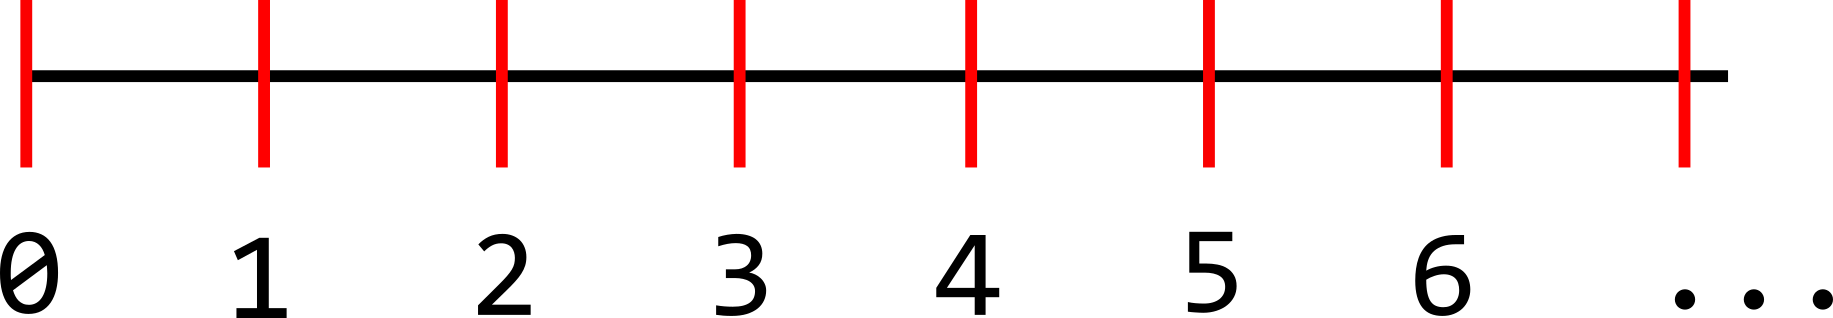
\includegraphics[height=.2\textheight]{resources/int_numbers.png}
  \end{center}
  
  \pause
  
  \texttt{int}

  \begin{center}
  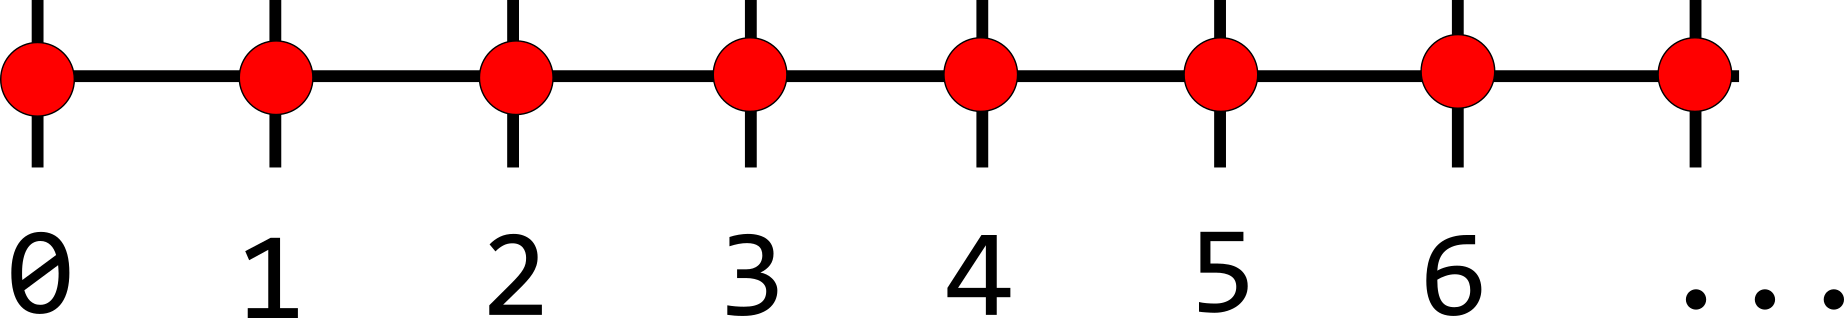
\includegraphics[height=.2\textheight]{resources/int_numbers_sampled.png}
  \end{center}
\end{frame}

\begin{frame}
  \frametitle{\texttt{float}s are different}
  
  $\mathbb{R}$
  
  \begin{center}
  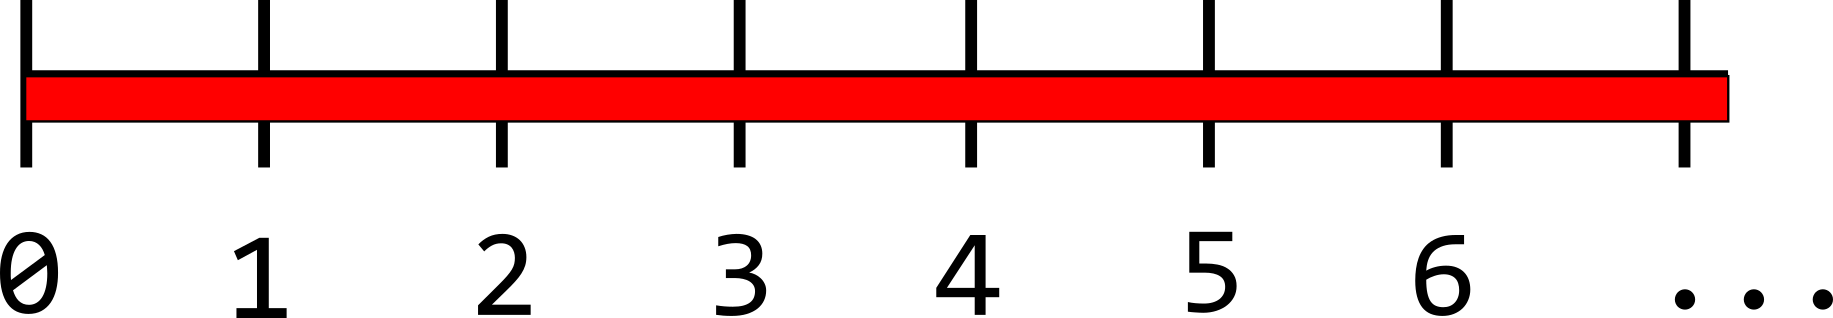
\includegraphics[height=.2\textheight]{resources/real_numbers.png}
  \end{center}
  
  \pause
  
  \texttt{float}

  \begin{center}
  ???
  \end{center}
\end{frame}


\begin{frame}
  \frametitle{\texttt{float}s are different}
  \texttt{float}

  \begin{center}
  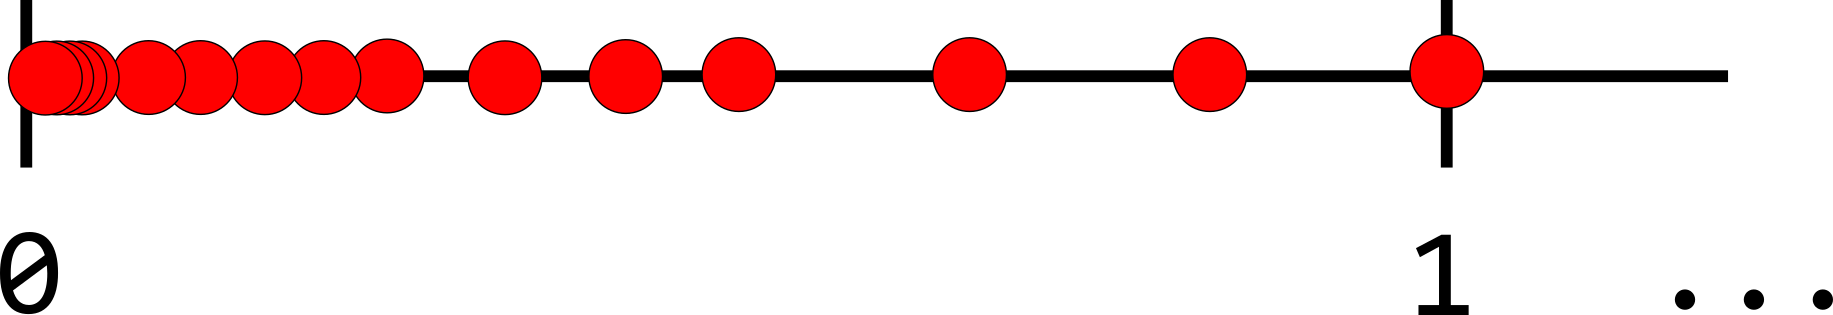
\includegraphics[height=.2\textheight]{resources/real_numbers_sampled.png}
  \end{center}
\end{frame}

\begin{frame}
  \frametitle{\texttt{float}s are different}
  \texttt{float}

  \begin{center}
  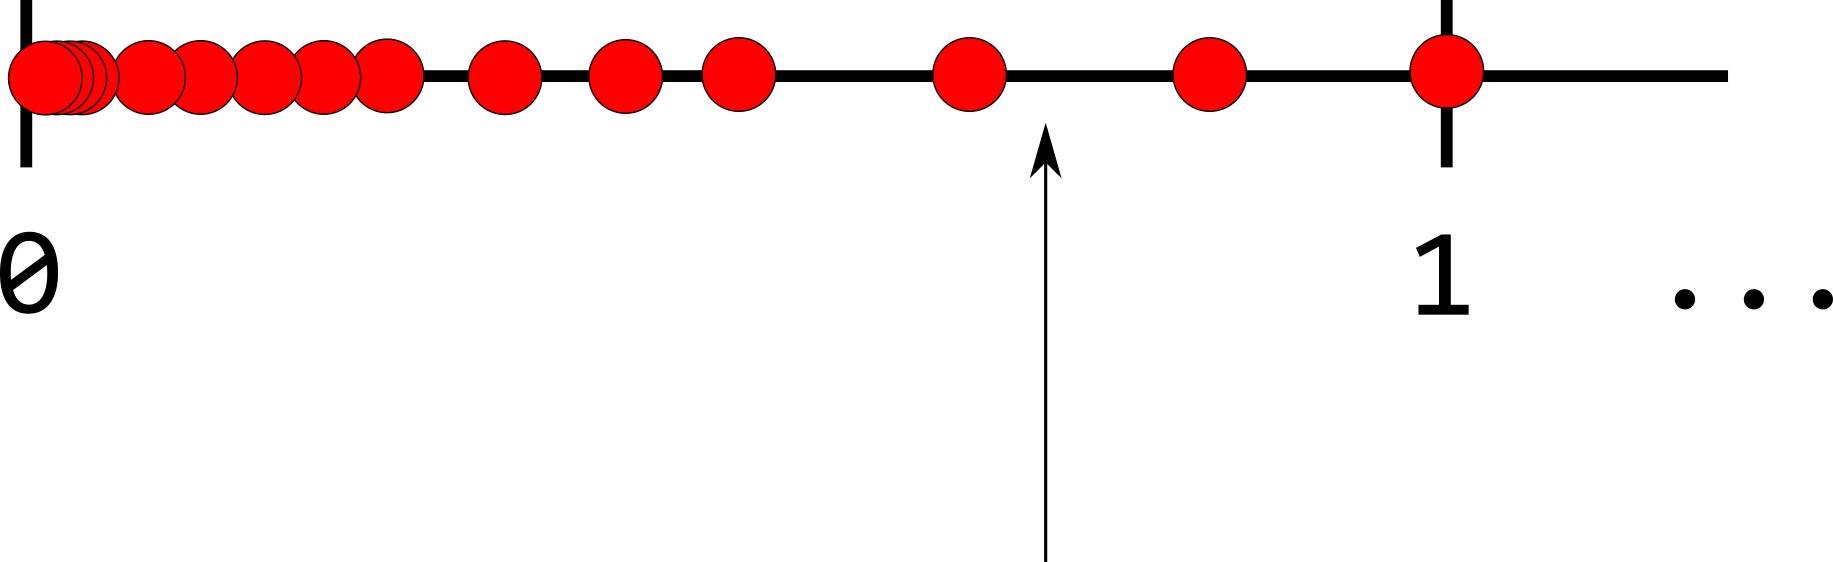
\includegraphics[height=.3547\textheight]{resources/real_numbers_sample_1.png}
  \end{center}
\end{frame}

\begin{frame}
  \frametitle{\texttt{float}s are different}
  \texttt{float}

  \begin{center}
  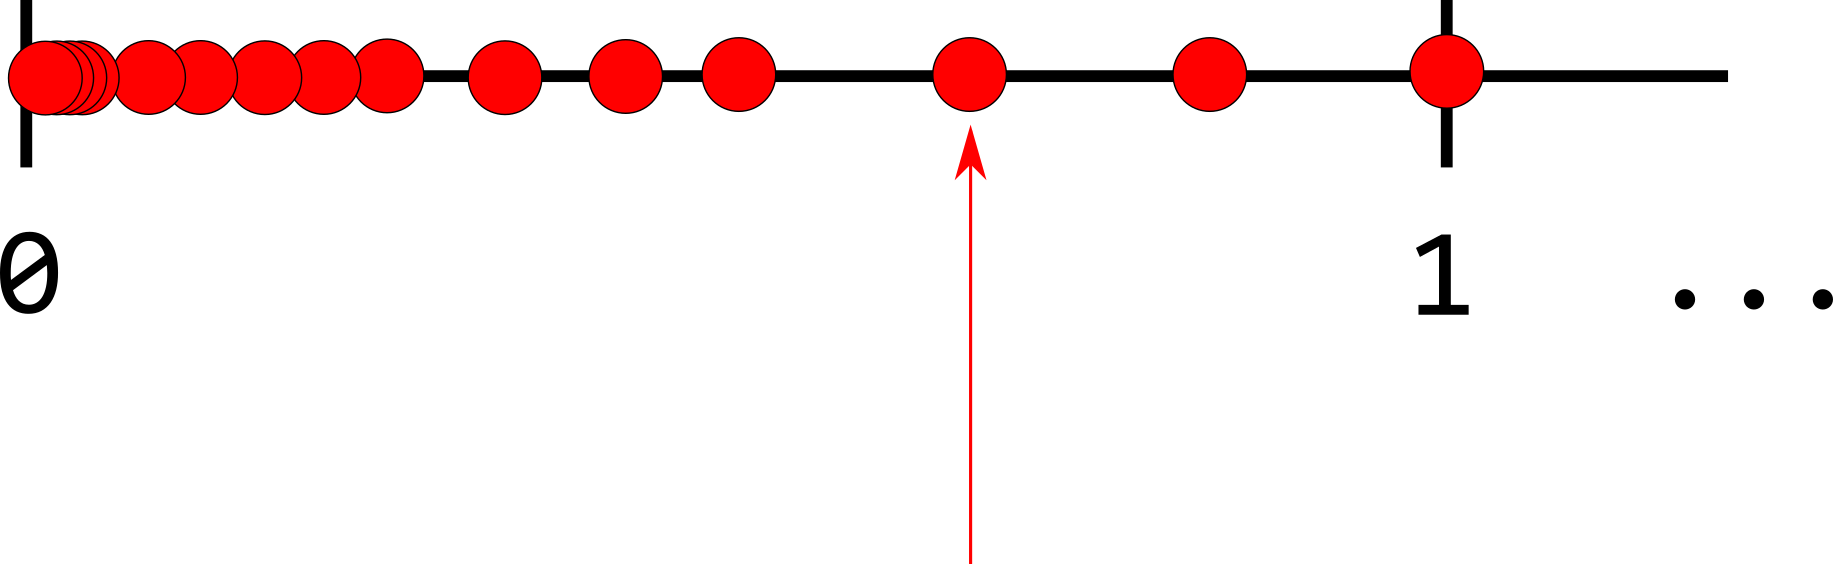
\includegraphics[height=.3547\textheight]{resources/real_numbers_sample_2.png}
  \end{center}
\end{frame}

\begin{frame}[fragile]
  \frametitle{\texttt{float}s are different}
    \begin{lstlisting}
double calc(std::vector<double> const& vd)
{
  double acc1 = 0.0, acc2 = 0.0;
  for(size_t i = 0; i < vd.size(); i += 2) {
    acc1 += vd[i]     * vd[i];
    acc2 += vd[i + 1] * vd[i + 1];
  }
  return acc1 + acc2;
}
    \end{lstlisting}
\end{frame}

\begin{frame}[fragile]
  \frametitle{With the right numbers...}
    \begin{lstlisting}
std::vector<double> input(1024*1024 * 128);
std::mt19937_64 rnd(42);

std::generate(begin(input), end(input),
  [&rnd]() {
    std::uniform_real_distribution<double>
      dist(0.0, 1.0e20);
    return dist(rnd);
  });
\end{lstlisting}

Result on \texttt{inner\_product} will be in the order of \texttt{4.47e+47}.
\end{frame}


\begin{frame}[fragile]
  \frametitle{\ldots differences start to appear}
  \texttt{Ryzen 7 1700X, g++ 8.1.1, -O3}
    \begin{lstlisting}
Naive version
124ms.
123ms.
126ms.
std::inner_product
123ms. (No difference.)
123ms. (No difference.)
123ms. (No difference.)
Unrolled
77ms. (Mismatch! Diff: -1.96171e+35)
82ms. (Mismatch! Diff: -1.96171e+35)
82ms. (Mismatch! Diff: -1.96171e+35)
    \end{lstlisting}
\end{frame}


\begin{frame}[fragile]
  \frametitle{Whereas with \texttt{-ffast-math}\ldots}
  \texttt{Ryzen 7 1700X, g++ 8.1.1, -O3 {\color{red}-ffast-math}}
    \begin{lstlisting}
Naive version
73ms.
76ms.
75ms.
std::inner_product
75ms. (No difference.)
74ms. (No difference.)
75ms. (No difference.)
Unrolled
76ms. (No difference.)
77ms. (No difference.)
76ms. (No difference.)
    \end{lstlisting}
\end{frame}

\begin{frame}
  \frametitle{On a related note}

  \begin{block}{From the cppreference page for std::inner\_product\footnote{https://en.cppreference.com/w/cpp/algorithm/inner\_product}}
  The parallelizable version of this algorithm, \texttt{std::transform\_reduce}, requires op1 and op2 to be {\color{red}commutative and associative}, but \texttt{std::inner\_product} makes no such requirement, and always performs the operations in the order given. 
  \end{block}
\end{frame}


\begin{frame}
  \frametitle{Thanks for your attention.}
\end{frame}


\end{document}
